
%(BEGIN_QUESTION)
% Copyright 2009, Tony R. Kuphaldt, released under the Creative Commons Attribution License (v 1.0)
% This means you may do almost anything with this work of mine, so long as you give me proper credit

Suppose you walk up to this thermocouple, installed to measure the temperature of an enclosed process vessel, and connect a sensitive voltmeter to the terminals at the junction head:

$$\includegraphics[width=15.5cm]{i04003x01.eps}$$

First, determine which lead of the voltmeter should contact which lead of the thermocouple (red to red?), then determine the temperature of the process vessel if the measured voltage is 15.830 mV.

\vskip 10pt

\vskip 20pt \vbox{\hrule \hbox{\strut \vrule{} {\bf Suggestions for Socratic discussion} \vrule} \hrule}

\begin{itemize}
\item{} Will the transmitter's measurement of temperature be affected when the voltmeter probes touch the thermocouple leads?  In other words, will this influence the temperature measurement for an operator (or an automatic controller) during your test?
\item{} Suppose the technician touches the multimeter probe tips to the thermocouple wires directly, rather than to the copper terminals inside the junction head.  Will this make any difference in the measurement?  Explain why or why not.
\item{} Suppose the technician mistakenly sets the multimeter up to measure {\it current} instead of voltage.  Will this affect the transmitter's measurement of temperature when the meter probes touch the thermocouple leads?
\end{itemize}

\underbar{file i04003}
%(END_QUESTION)





%(BEGIN_ANSWER)

\noindent
{\bf Partial answer:}

\vskip 10pt

The {\it red} test lead of the meter (+) should contact the {\it violet} wire of the thermocouple.  The {\it black} test lead of the meter ($-$) should contact the {\it red} wire of the thermocouple.

\vskip 10pt

An equivalent circuit diagram shows the relationship between the thermocouple measurement junction (in the process), the two reference junctions formed where thermocouple wire meets copper wire, the digital multimeter, and the temperature transmitter:

$$\includegraphics[width=15.5cm]{i04003x02.eps}$$

If your answer was 480 $^{o}$F or 481 $^{o}$F, you made a common mistake, which is correctable by close examination of the above diagram!

%(END_ANSWER)





%(BEGIN_NOTES)

This, of course, is a type E thermocouple.

\vskip 10pt

Connecting the copper test leads of the voltmeter to the thermocouple leads at the junction ``head'' creates a reference junction for the voltmeter circuit at that head location.  Therefore the ambient temperature at the head (87 $^{o}$F) becomes relevant for the voltmeter while the temperature at the transmitter is not.  The transmitter's ambient temperature is of course still relevant for the transmitter, because that's where the {\it transmitter's} reference junction is located.

Knowing that the voltmeter will register the {\it difference} in voltage between the measurement junction and its reference junction, and knowing that the voltage produced by a type E reference junction at 87 $^{o}$F is 1.835 mV, we must {\it add} the voltmeter's reading of 15.830 mV to the table-referenced junction voltage of 1.835 mV to get a measurement junction voltage of 17.665 mV, which corresponds to a temperature {\bf between 493 $^{o}$F and 494 $^{o}$F}.

%INDEX% Measurement, temperature: thermocouple millivoltage interpretation

%(END_NOTES)


